Comparing generated energy reported in the \ac{MER} Opportunity status update logs to those predicted by Equation \ref{eq:SA_energy} resulted in a -33\%/+7\% error margin range. This range can be narrowed down and shifted by adjusting the reported solar array dust factor as well as the assumptions made for shadowing and other losses. Reported $\tau$ factors are kept as is.

\section{Preserving Outliers}
\label{sec:Appendix:NarrowedEnergyPredictionErrorMarginRange:PreservingOutliers}

The margin of error range is narrowed by selecting a target range and applying corrective coefficients to the reported solar array dust factor in combination with revised performance degradation factors pertaining to shadowing and other losses. Table \ref{tab:target-error-margins} presents the adjustment coefficients that were iteratively obtained. Shadowing and other losses was constrained based on the assumption that they cumulatively range from 5\% to 7\%.

Negative error margin values correspond to over-estimated daily energy predictions, hence the -10\%/+25\% range is preferred in order to limit over-estimations. From the possible combinations of dust factor adjustment with shadowing and other losses, the option with the smallest dust factor adjustment is preferred so to not rely on large changes of the reported duct factor to calibrate Equation \ref{eq:SA_energy}.

\begin{table}[h]
\centering
\caption{Combination of shadowing and other losses with solar array dust factor adjustment coefficients to obtain different error margin ranges. }
\label{tab:target-error-margins}
\begin{tabular}{|c|c|c|}
\hline
\textbf{\begin{tabular}[c]{@{}c@{}}Error\\ Margins\\ Ranges\end{tabular}} & \textbf{\begin{tabular}[c]{@{}c@{}}Shadowing\\ and\\ Other Losses\end{tabular}} & \textbf{\begin{tabular}[c]{@{}c@{}}Solar Array\\ Dust Factor\\ Adjustment\end{tabular}} \\ \hline
\multirow{3}{*}{-20\% / +18\%} & 5\% & 7.5\% \\ \cline{2-3}
 & 6\% & 5.5\% \\ \cline{2-3}
 & 7\% & 3.5\% \\ \hhline{|=|=|=|}
\multirow{3}{*}{-15\% / +21\%} & 5\% & 10.3\% \\ \cline{2-3}
 & 6\% & 8.3\% \\ \cline{2-3}
 & 7\% & 6.3\% \\ \hhline{|=|=|=|}
\multirow{3}{*}{-14\% / +22\%} & 5\% & 10.8\% \\ \cline{2-3}
 & 6\% & 8.8\% \\ \cline{2-3}
 & 7\% & 6.3\% \\ \hhline{|=|=|=|}
\multirow{3}{*}{-13\% / +23\%} & 5\% & 11.4\% \\ \cline{2-3}
 & 6\% & 9.4\% \\ \cline{2-3}
 & 7\% & 7.4\% \\ \hhline{|=|=|=|}
\multirow{3}{*}{-12\% / +23\%} & 5\% & 11.9\% \\ \cline{2-3}
 & 6\% & 9.9\% \\ \cline{2-3}
 & 7\% & 7.9\% \\ \hhline{|=|=|=|}
\multirow{3}{*}{-11\% / +24\%} & 5\% & 12.5\% \\ \cline{2-3}
 & 6\% & 10.5\% \\ \cline{2-3}
 & 7\% & 8.5\% \\ \hhline{|=|=|=|}
\multirow{3}{*}{-10\% / +25\%} & 5\% & 13.1\% \\ \cline{2-3}
 & 6\% & 11.1\% \\ \cline{2-3}
 & 7\% & 9.1\% \\ \hline
\end{tabular}
\end{table}


\clearpage
Applying a 9.1\% dust factor adjustment coupled with a 7\% shadowing and other losses results in the adjusted divergences presented in Figure \ref{fig:plot:mer-energy-prediction-divergences-adjusted}:

\begin{figure}[h]
  \centering
  \hypersetup{linkcolor=captionTextColor}
  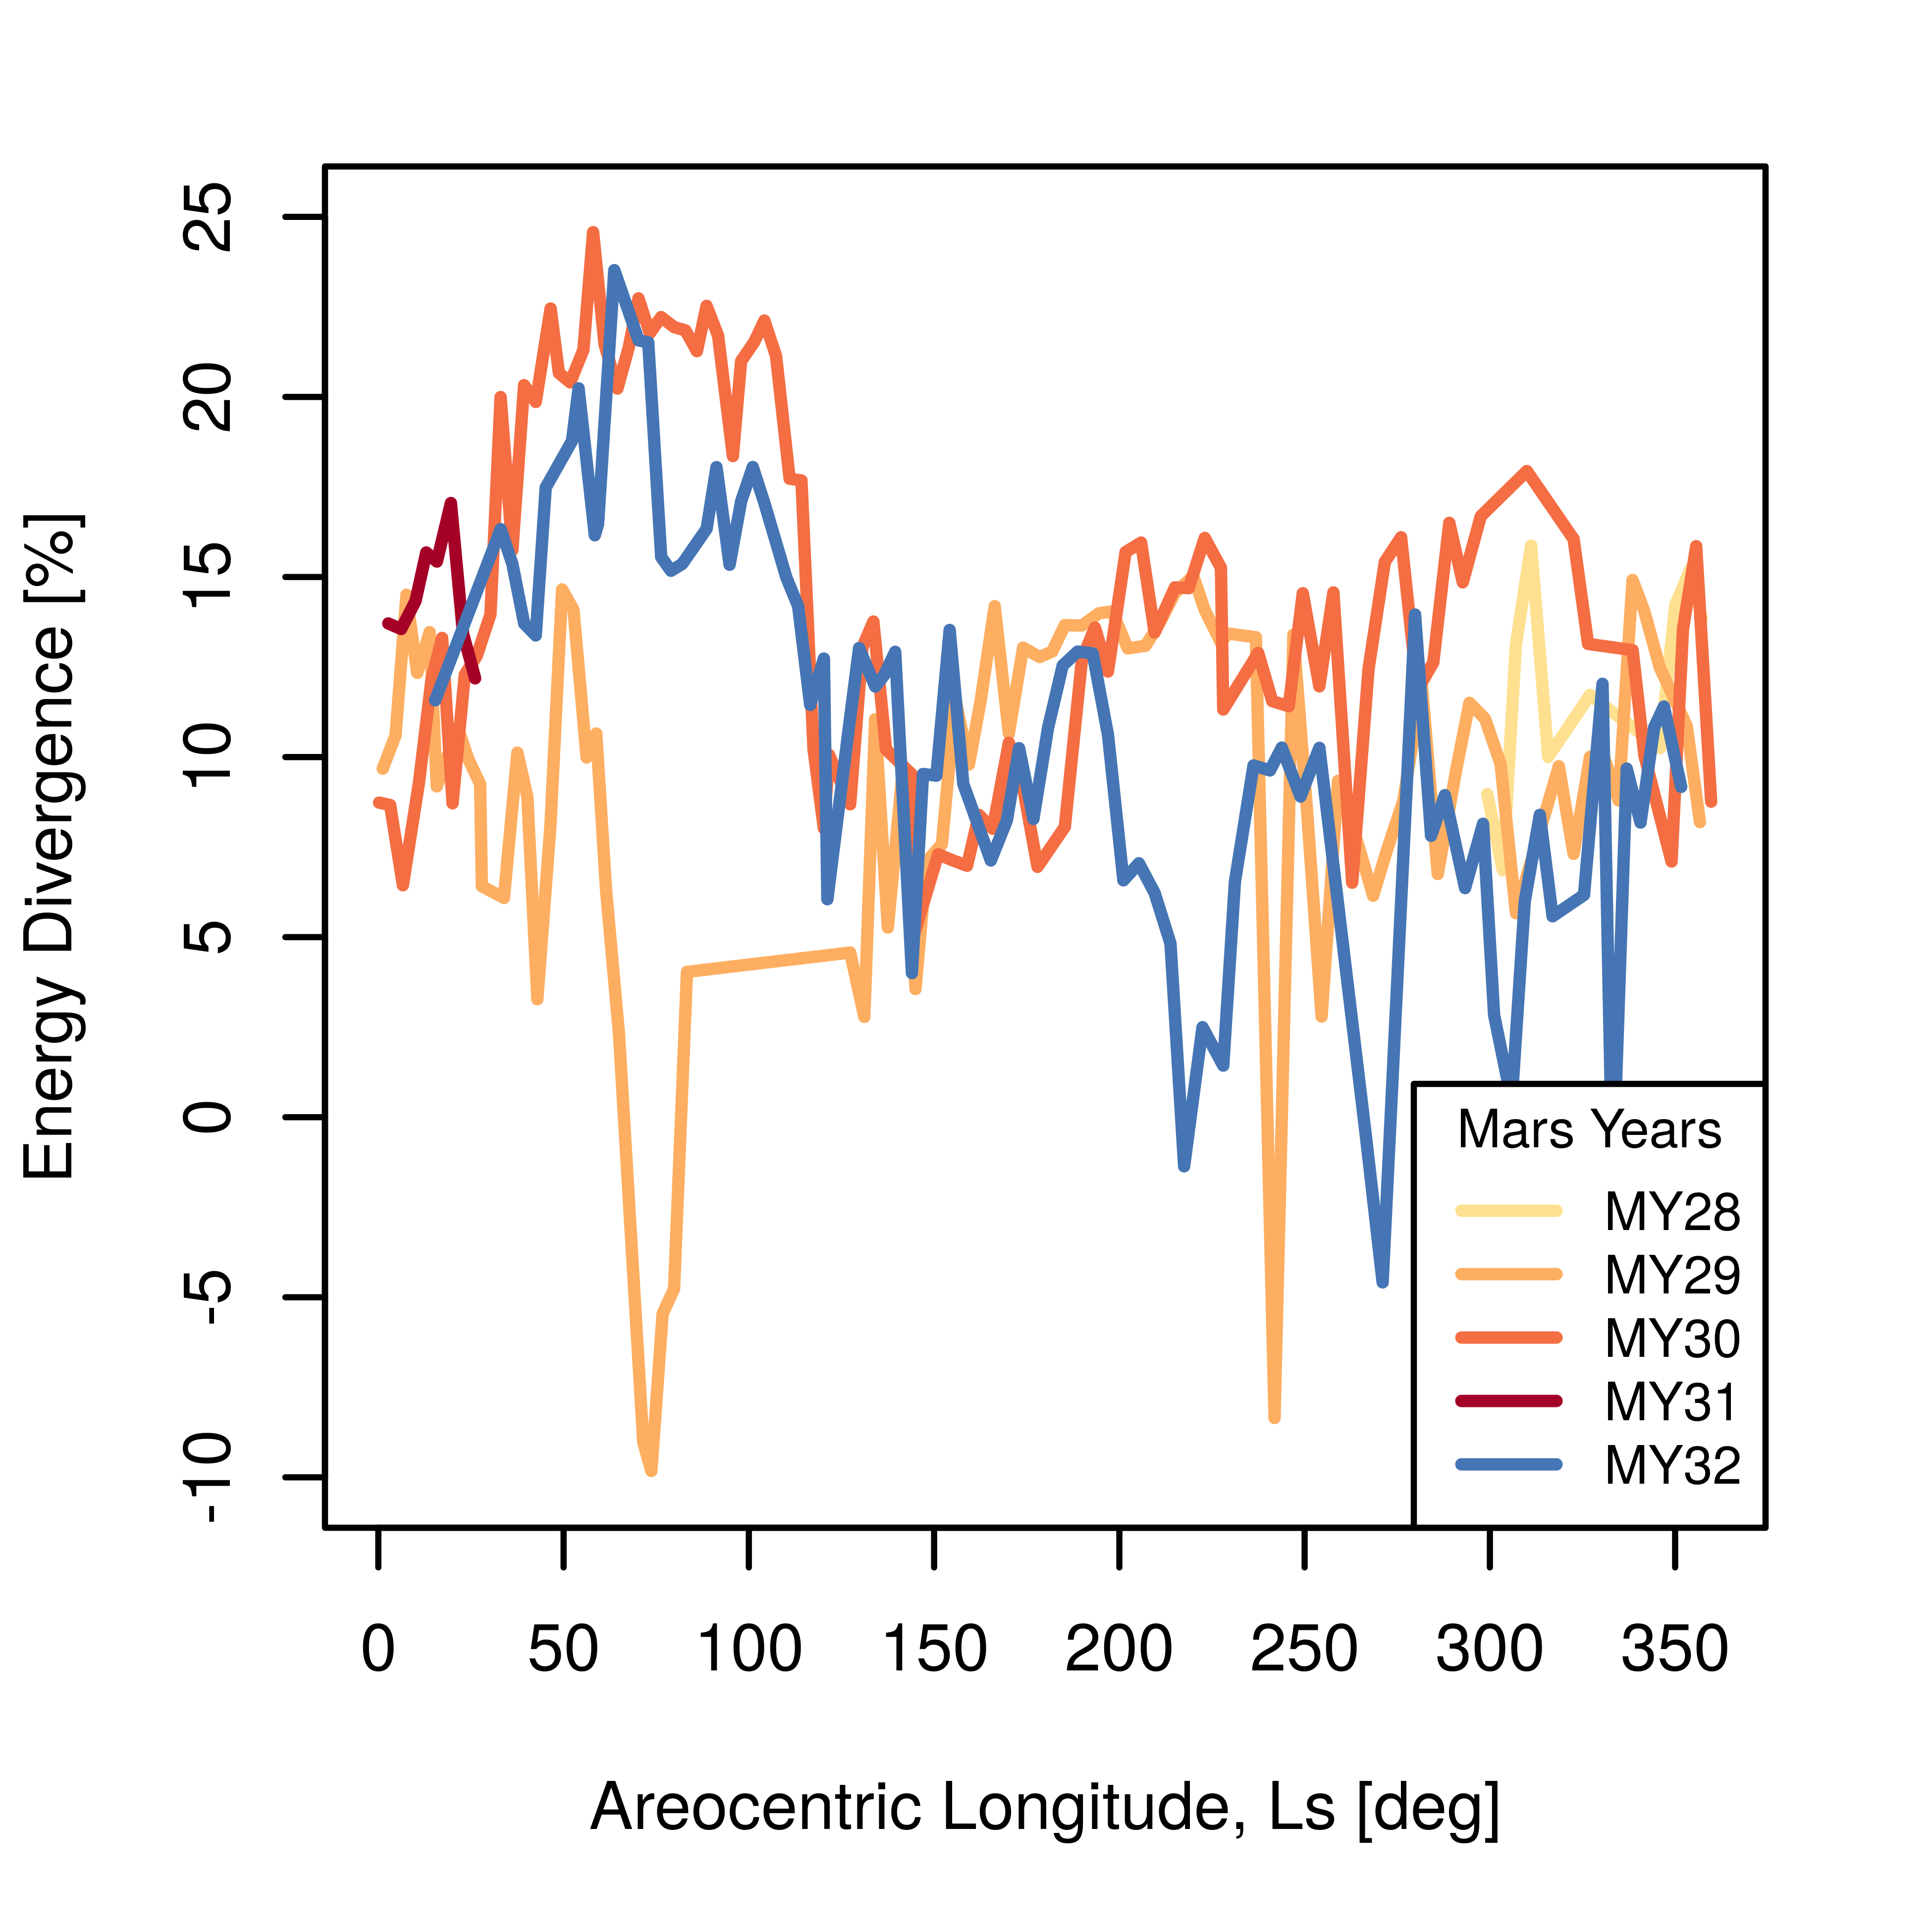
\includegraphics[width=0.8\linewidth]{sections/appendix/energy-error-margin/plots/energy-prediction-divergences-from-my28-to-my32-adjusted.png}\\
  \caption[Adjusted divergences from measured \ac{MER} Opportunity PV energy production]
          {Adjusted divergences from measured \ac{MER} Opportunity PV energy production.}
  \label{fig:plot:mer-energy-prediction-divergences-adjusted}
\end{figure}

\clearpage

\section{Ignoring Outliers}
\label{sec:Appendix:NarrowedEnergyPredictionErrorMarginRange:IgnoringOutliers}

In Figure \ref{fig:plot:binned-error-margins}, divergences greater than 5\% and lesser than -15\% were obtained with only 9.2\% of the dataset. With this in consideration, the process described in Section \ref{sec:Appendix:NarrowedEnergyPredictionErrorMarginRange:PreservingOutliers} was repeated without the data points responsible for the divergence outliers. This further narrowed down the error margin range to -11\%/+5\% by applying solar array dust factor adjustment of 5.4\% coupled with shadowing and other losses of 5\%. The resulting adjusted divergences are presented in Figure \ref{fig:plot:mer-energy-prediction-divergences-adjusted-without-outliers}:

\begin{figure}[h]
  \centering
  \hypersetup{linkcolor=captionTextColor}
  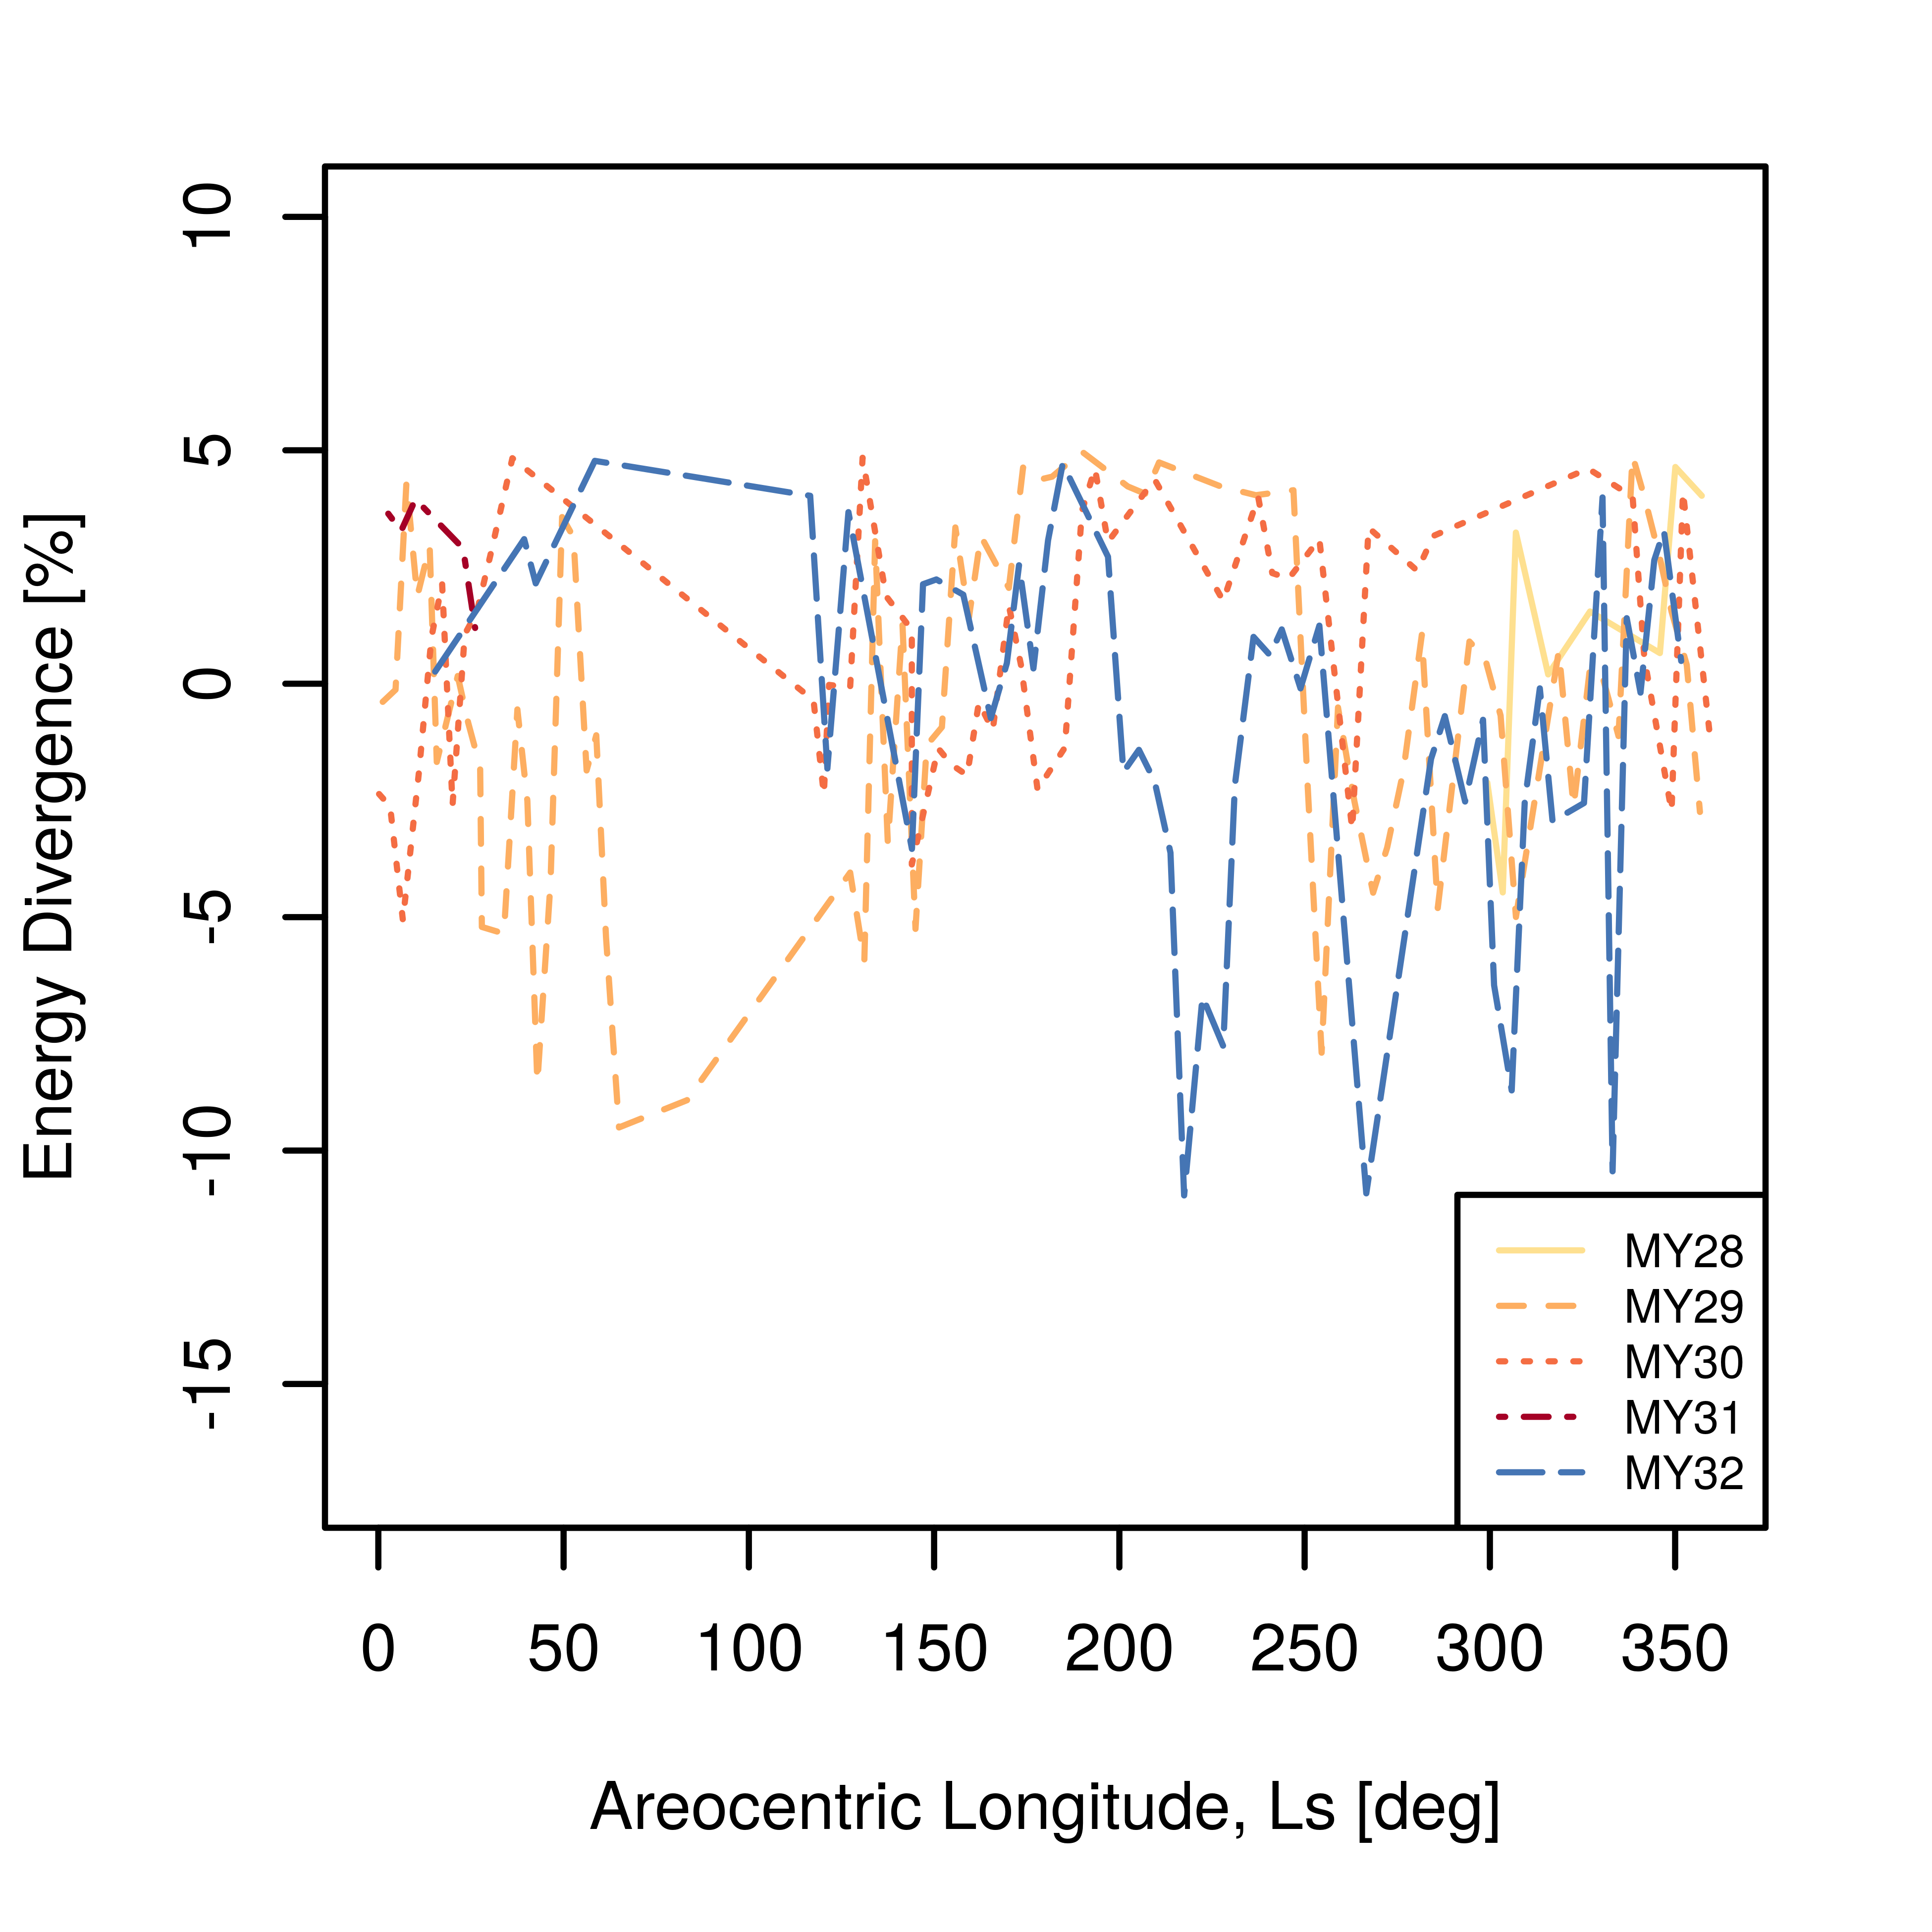
\includegraphics[width=0.8\linewidth]{sections/appendix/energy-error-margin/plots/energy-prediction-divergences-from-my28-to-my32-adjusted-without-outliers.png}\\
  \caption[Adjusted Outlierless divergences from measured \ac{MER} Opportunity PV energy production]
          {Adjusted Outlierless divergences from measured \ac{MER} Opportunity PV energy production.}
  \label{fig:plot:mer-energy-prediction-divergences-adjusted-without-outliers}
\end{figure}

\clearpage

\section{Conclusion}
\label{sec:Appendix:NarrowedEnergyPredictionErrorMarginRange:Conclusion}

The predicted generated energy curves in Figures \ref{fig:plot:sub:mer-energy-production-predicted-vs-reported-my29-adjusted}, \ref{fig:plot:sub:mer-energy-production-predicted-vs-reported-my30-adjusted}, and \ref{fig:plot:sub:mer-energy-production-predicted-vs-reported-my32-adjusted} were obtained through the process described in Section \ref{sec:Appendix:NarrowedEnergyPredictionErrorMarginRange:PreservingOutliers}. This resulted in overly conservative predictions when compared with the curve representing energy productions reported by MER Opportunity.

Predictions in Figures \ref{fig:plot:sub:mer-energy-production-predicted-vs-reported-my29-adjusted-without-outliers}, \ref{fig:plot:sub:mer-energy-production-predicted-vs-reported-my30-adjusted-without-outliers}, and \ref{fig:plot:sub:mer-energy-production-predicted-vs-reported-my32-adjusted-without-outliers} were obtained through the process described in Section \ref{sec:Appendix:NarrowedEnergyPredictionErrorMarginRange:IgnoringOutliers}. This resulted in predictions that more closely follow reported energy productions. Comparing these predictions with the unadjusted ones presented in Figure \ref{fig:plot:mer-energy-production-predicted-vs-reported} shows little changes and therefor do not justify the need to narrow down the error margin range for the purposes of preliminary mission scenario analysis.

\begin{figure}[h]
\captionsetup[subfigure]{justification=centering}
\vspace{-2ex}
	\centering
    %% setup sizes
    \setlength{\subfigureWidth}{0.32\textwidth}
    \setlength{\graphicsHeight}{50mm}
    %% kill hyper-link highlighting
    \hypersetup{hidelinks=true}%
    %% the figures
	\begin{subfigure}[t]{\subfigureWidth}
        \centering
		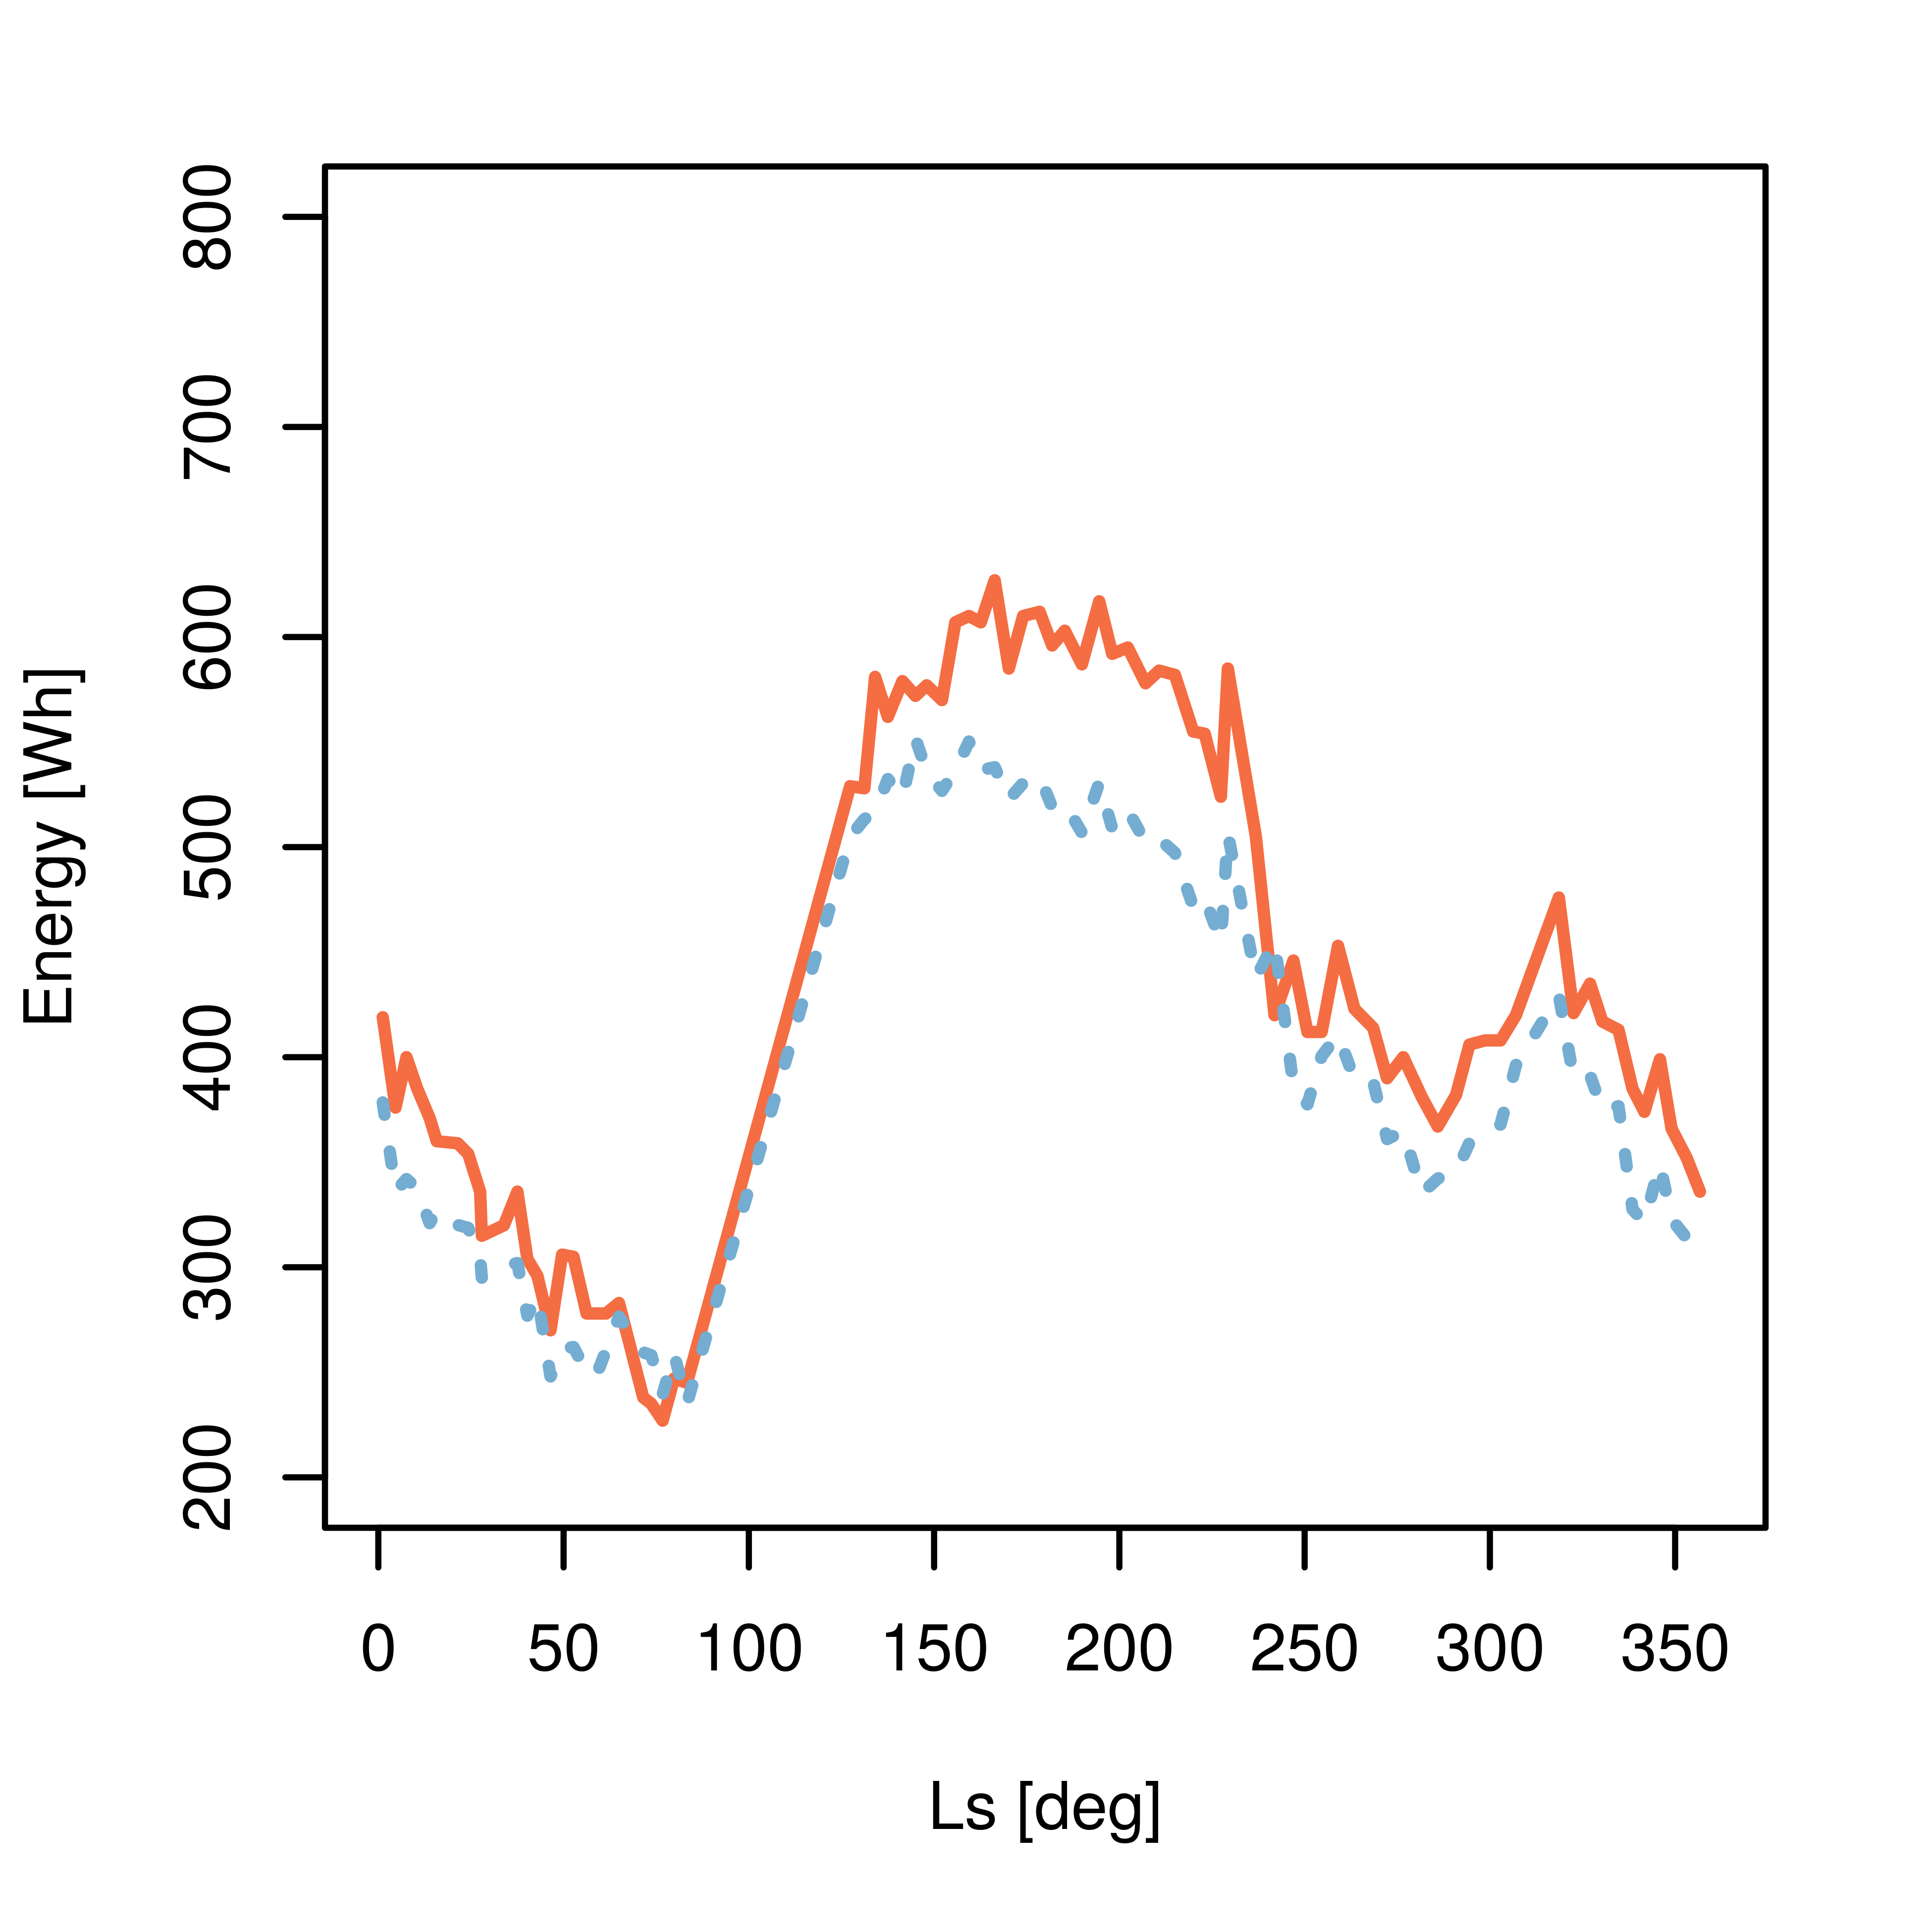
\includegraphics[height=\graphicsHeight]{sections/appendix/energy-error-margin/plots/predicted-vs-measured-energy-my29-adjusted.png}
		\subcaption{MY29}
		\label{fig:plot:sub:mer-energy-production-predicted-vs-reported-my29-adjusted}
	\end{subfigure}\hfill
	\begin{subfigure}[t]{\subfigureWidth}
        \centering
		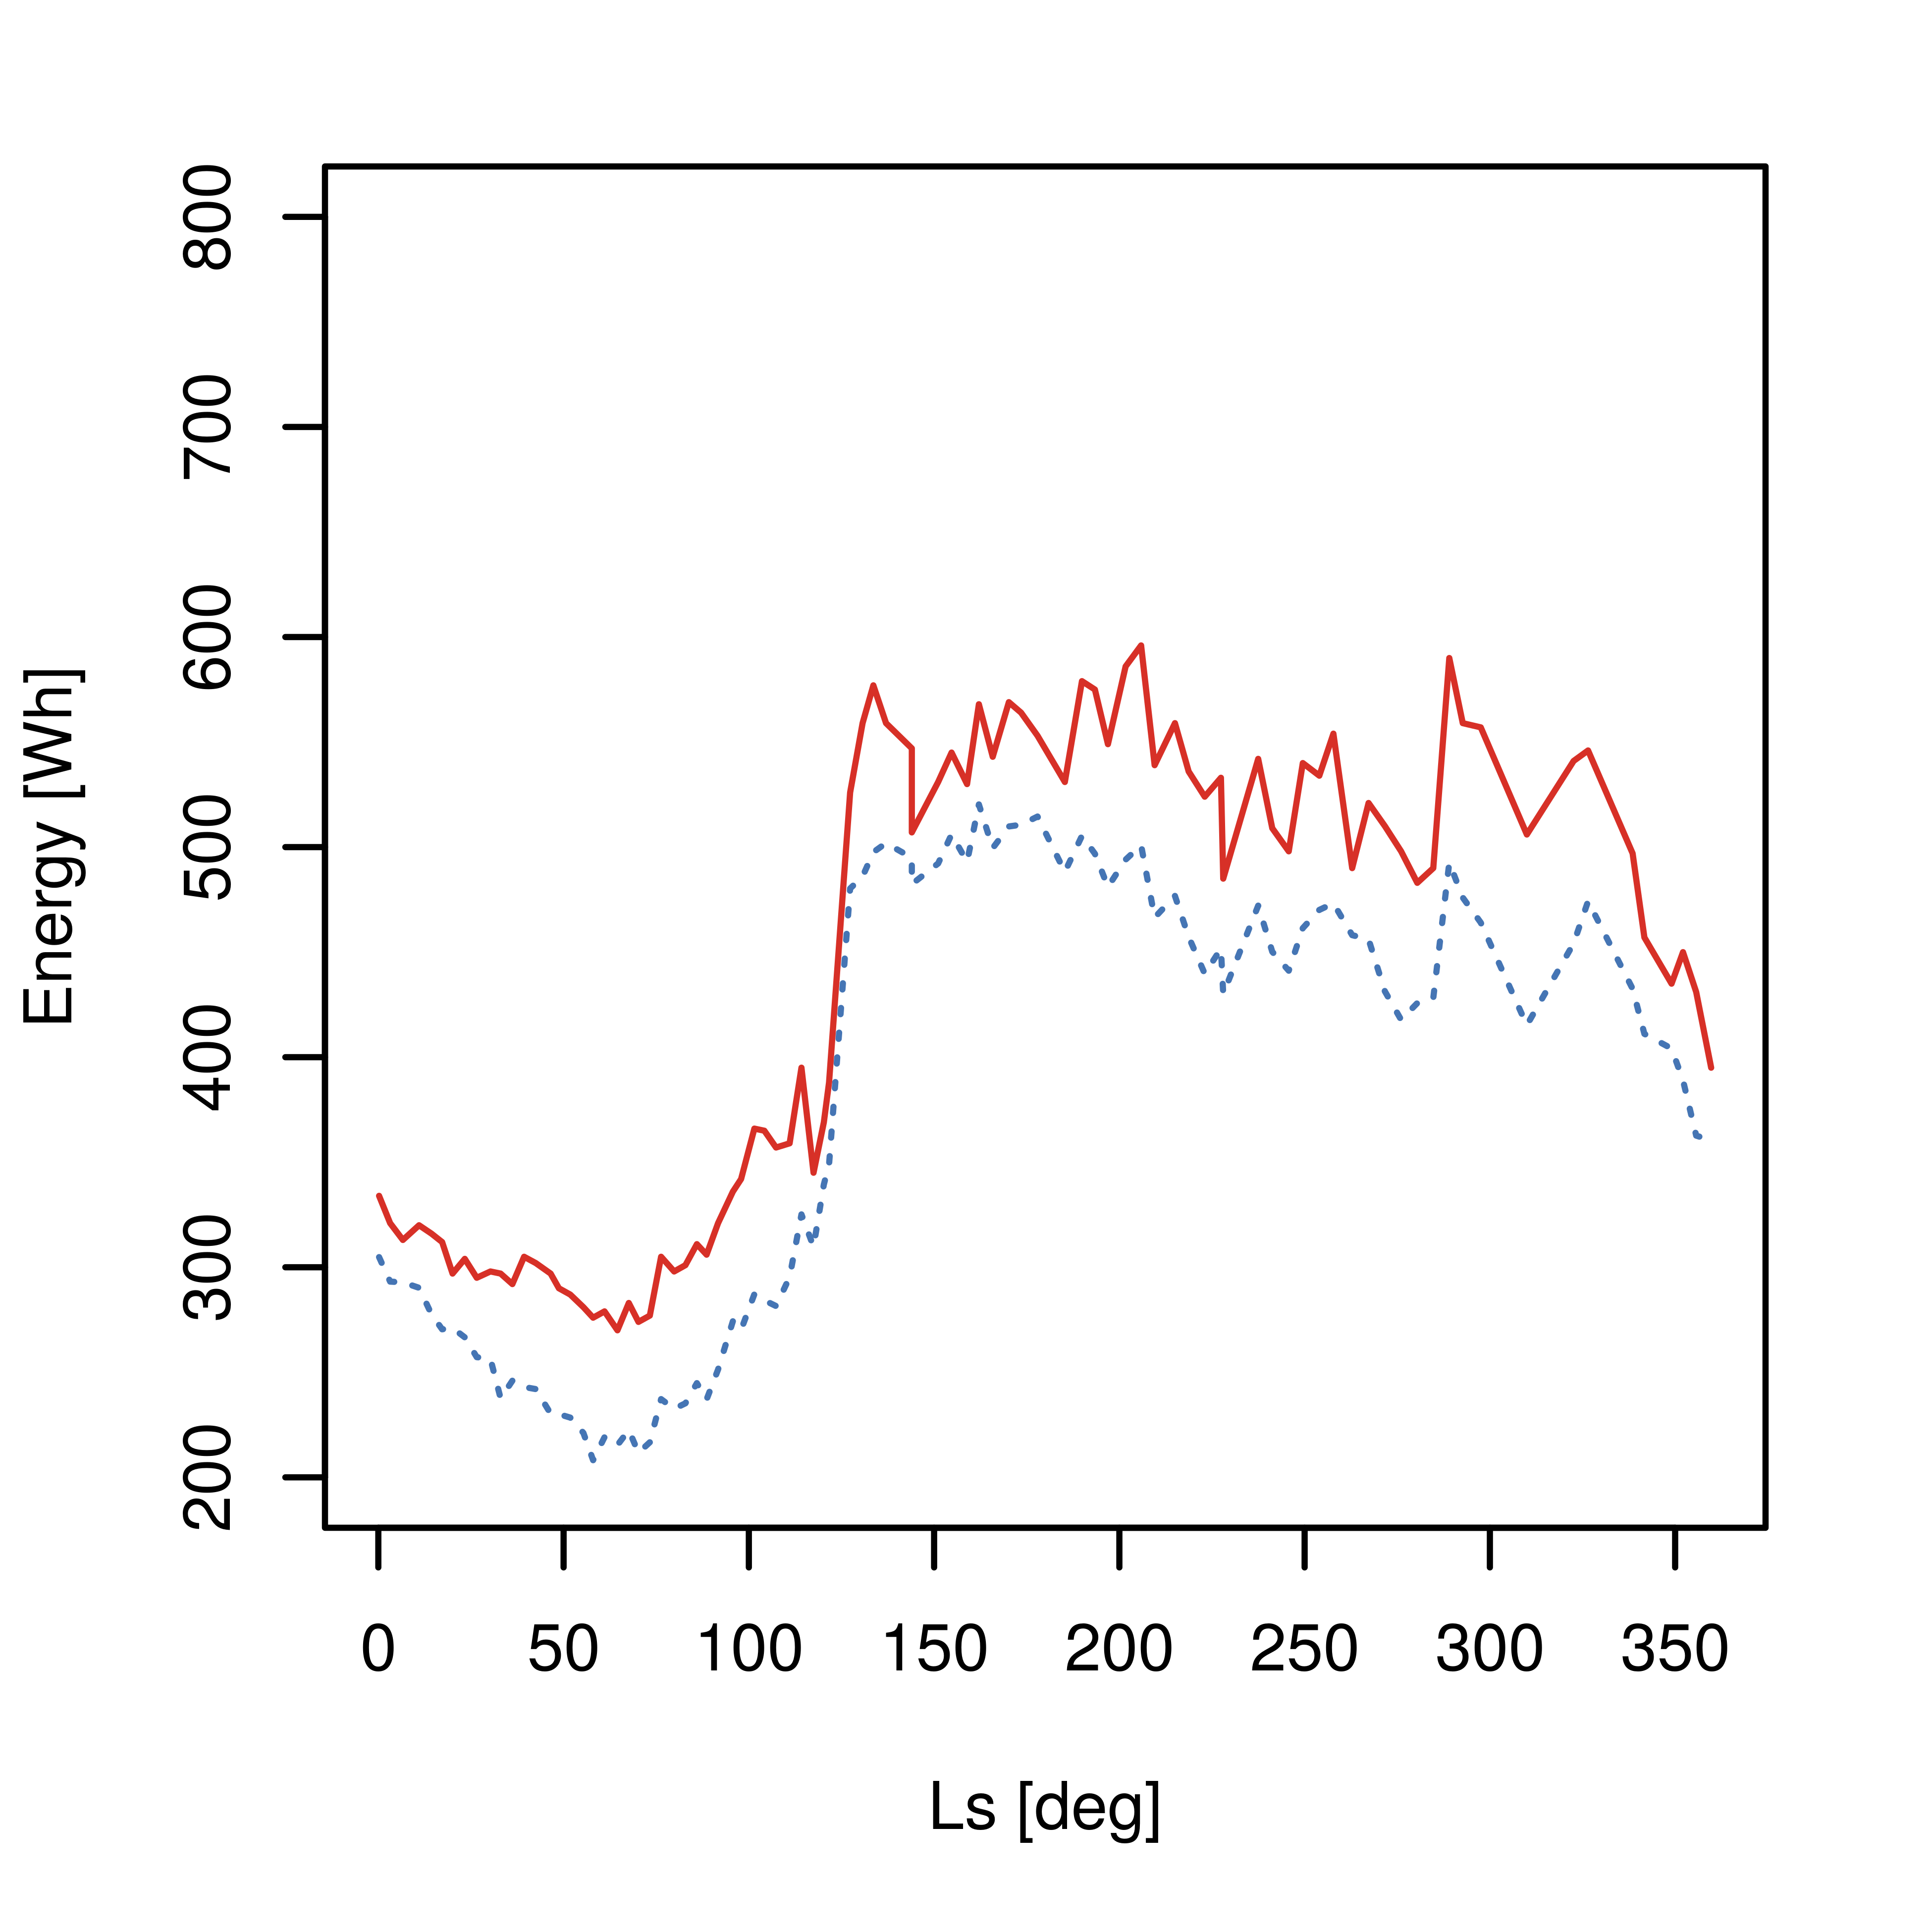
\includegraphics[height=\graphicsHeight]{sections/appendix/energy-error-margin/plots/predicted-vs-measured-energy-my30-adjusted.png}
		\subcaption{MY30}
		\label{fig:plot:sub:mer-energy-production-predicted-vs-reported-my30-adjusted}
	\end{subfigure}\hfill
    \begin{subfigure}[t]{\subfigureWidth}
        \centering
		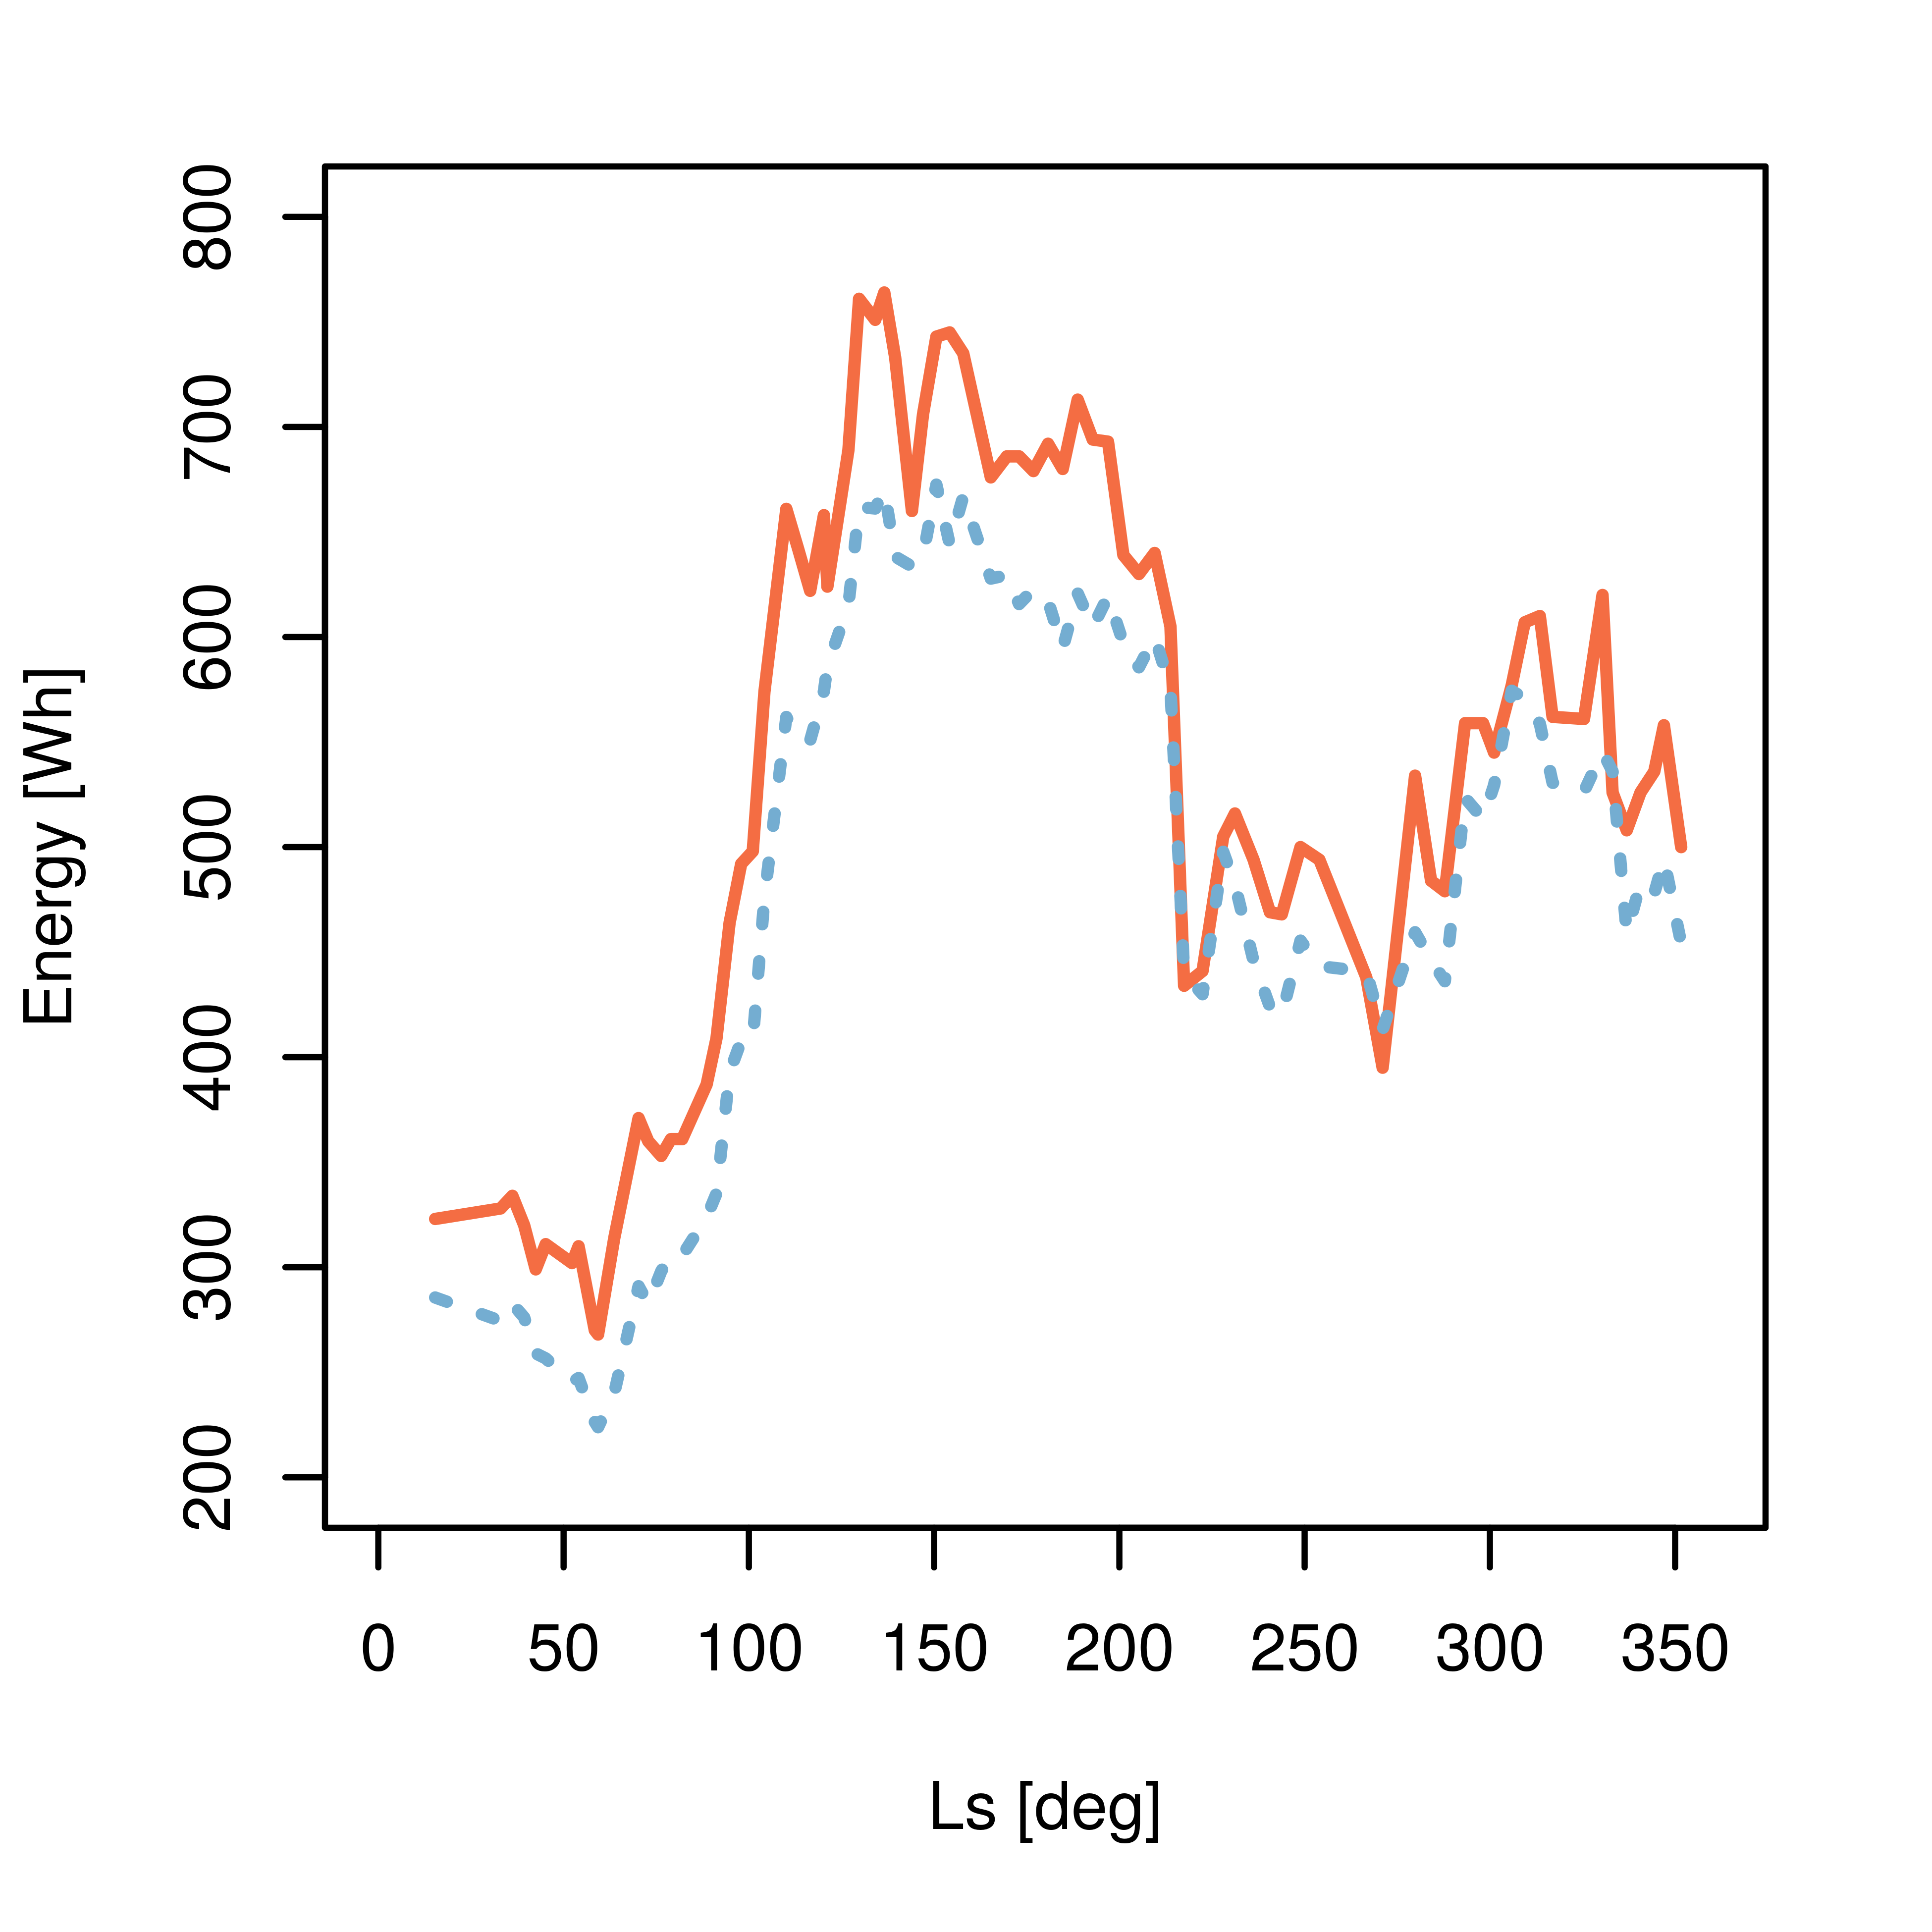
\includegraphics[height=\graphicsHeight]{sections/appendix/energy-error-margin/plots/predicted-vs-measured-energy-my32-adjusted.png}
		\subcaption{MY32}
		\label{fig:plot:sub:mer-energy-production-predicted-vs-reported-my32-adjusted}
	\end{subfigure}\\[0.8ex]
%% 2nd row
    \begin{subfigure}[t]{\subfigureWidth}
        \centering
		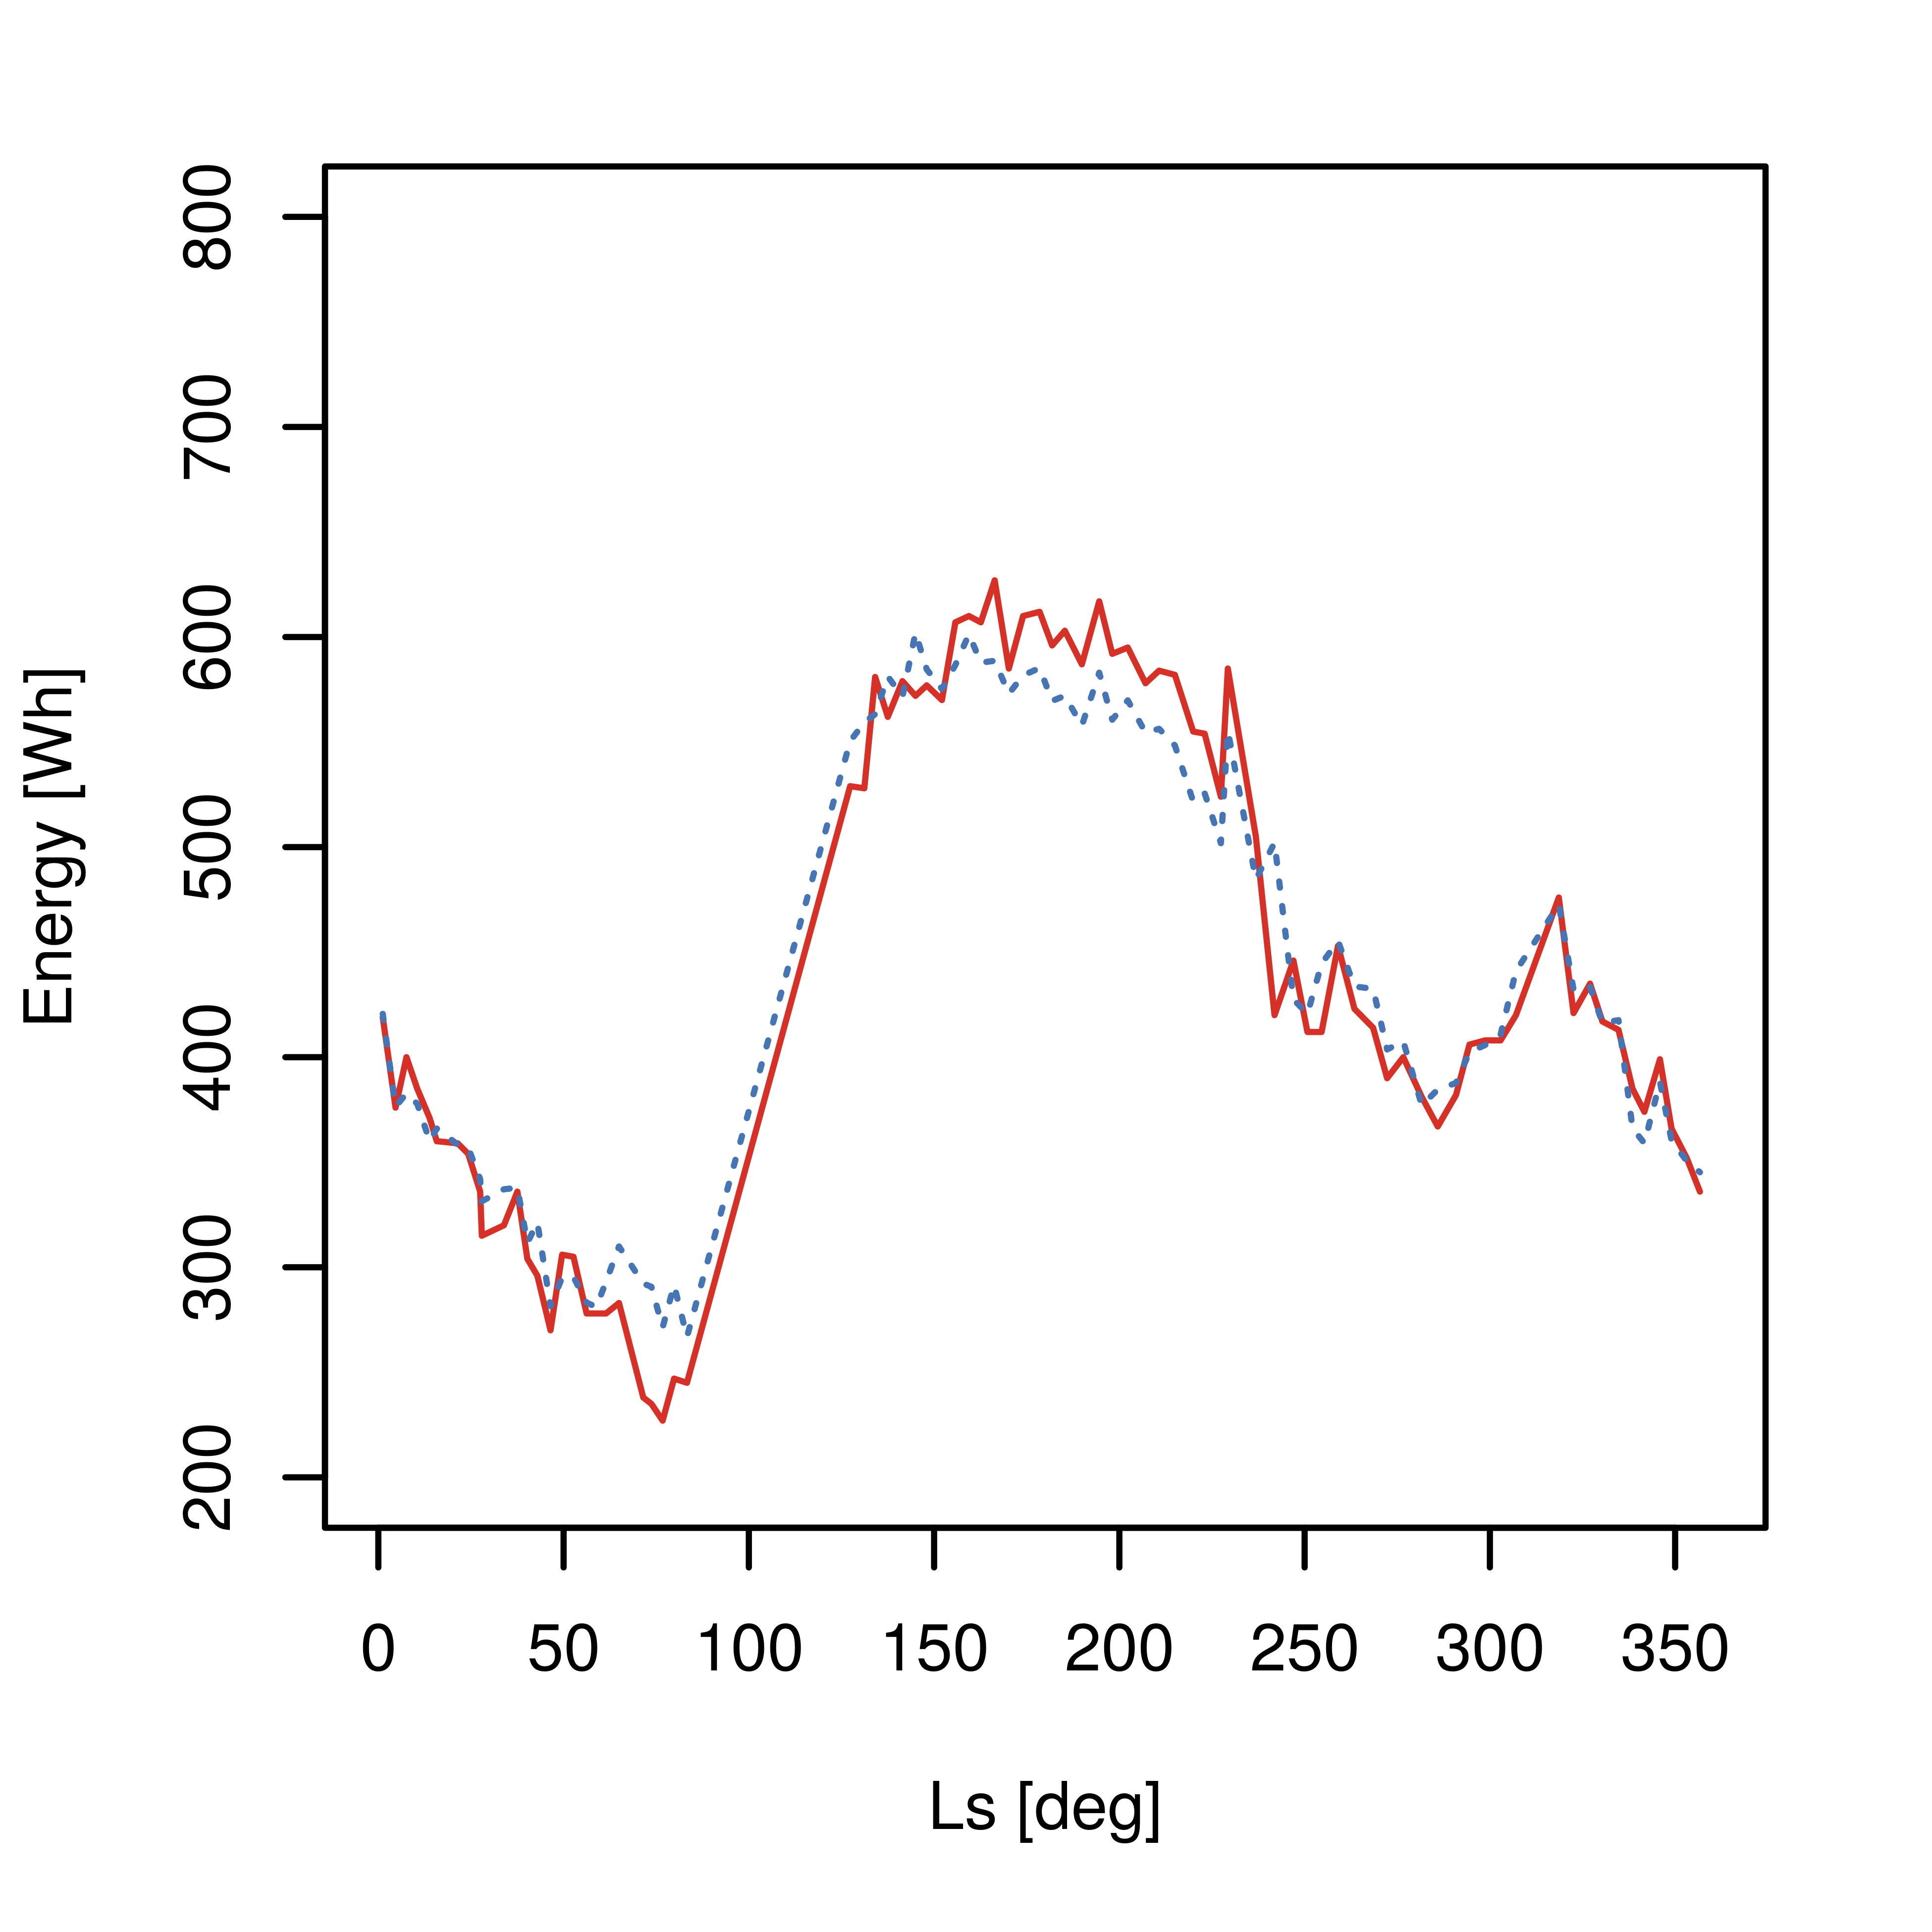
\includegraphics[height=\graphicsHeight]{sections/appendix/energy-error-margin/plots/predicted-vs-measured-energy-my29-adjusted-without-outliers.png}
		\subcaption{MY29}
		\label{fig:plot:sub:mer-energy-production-predicted-vs-reported-my29-adjusted-without-outliers}
	\end{subfigure}\hfill
	\begin{subfigure}[t]{\subfigureWidth}
        \centering
		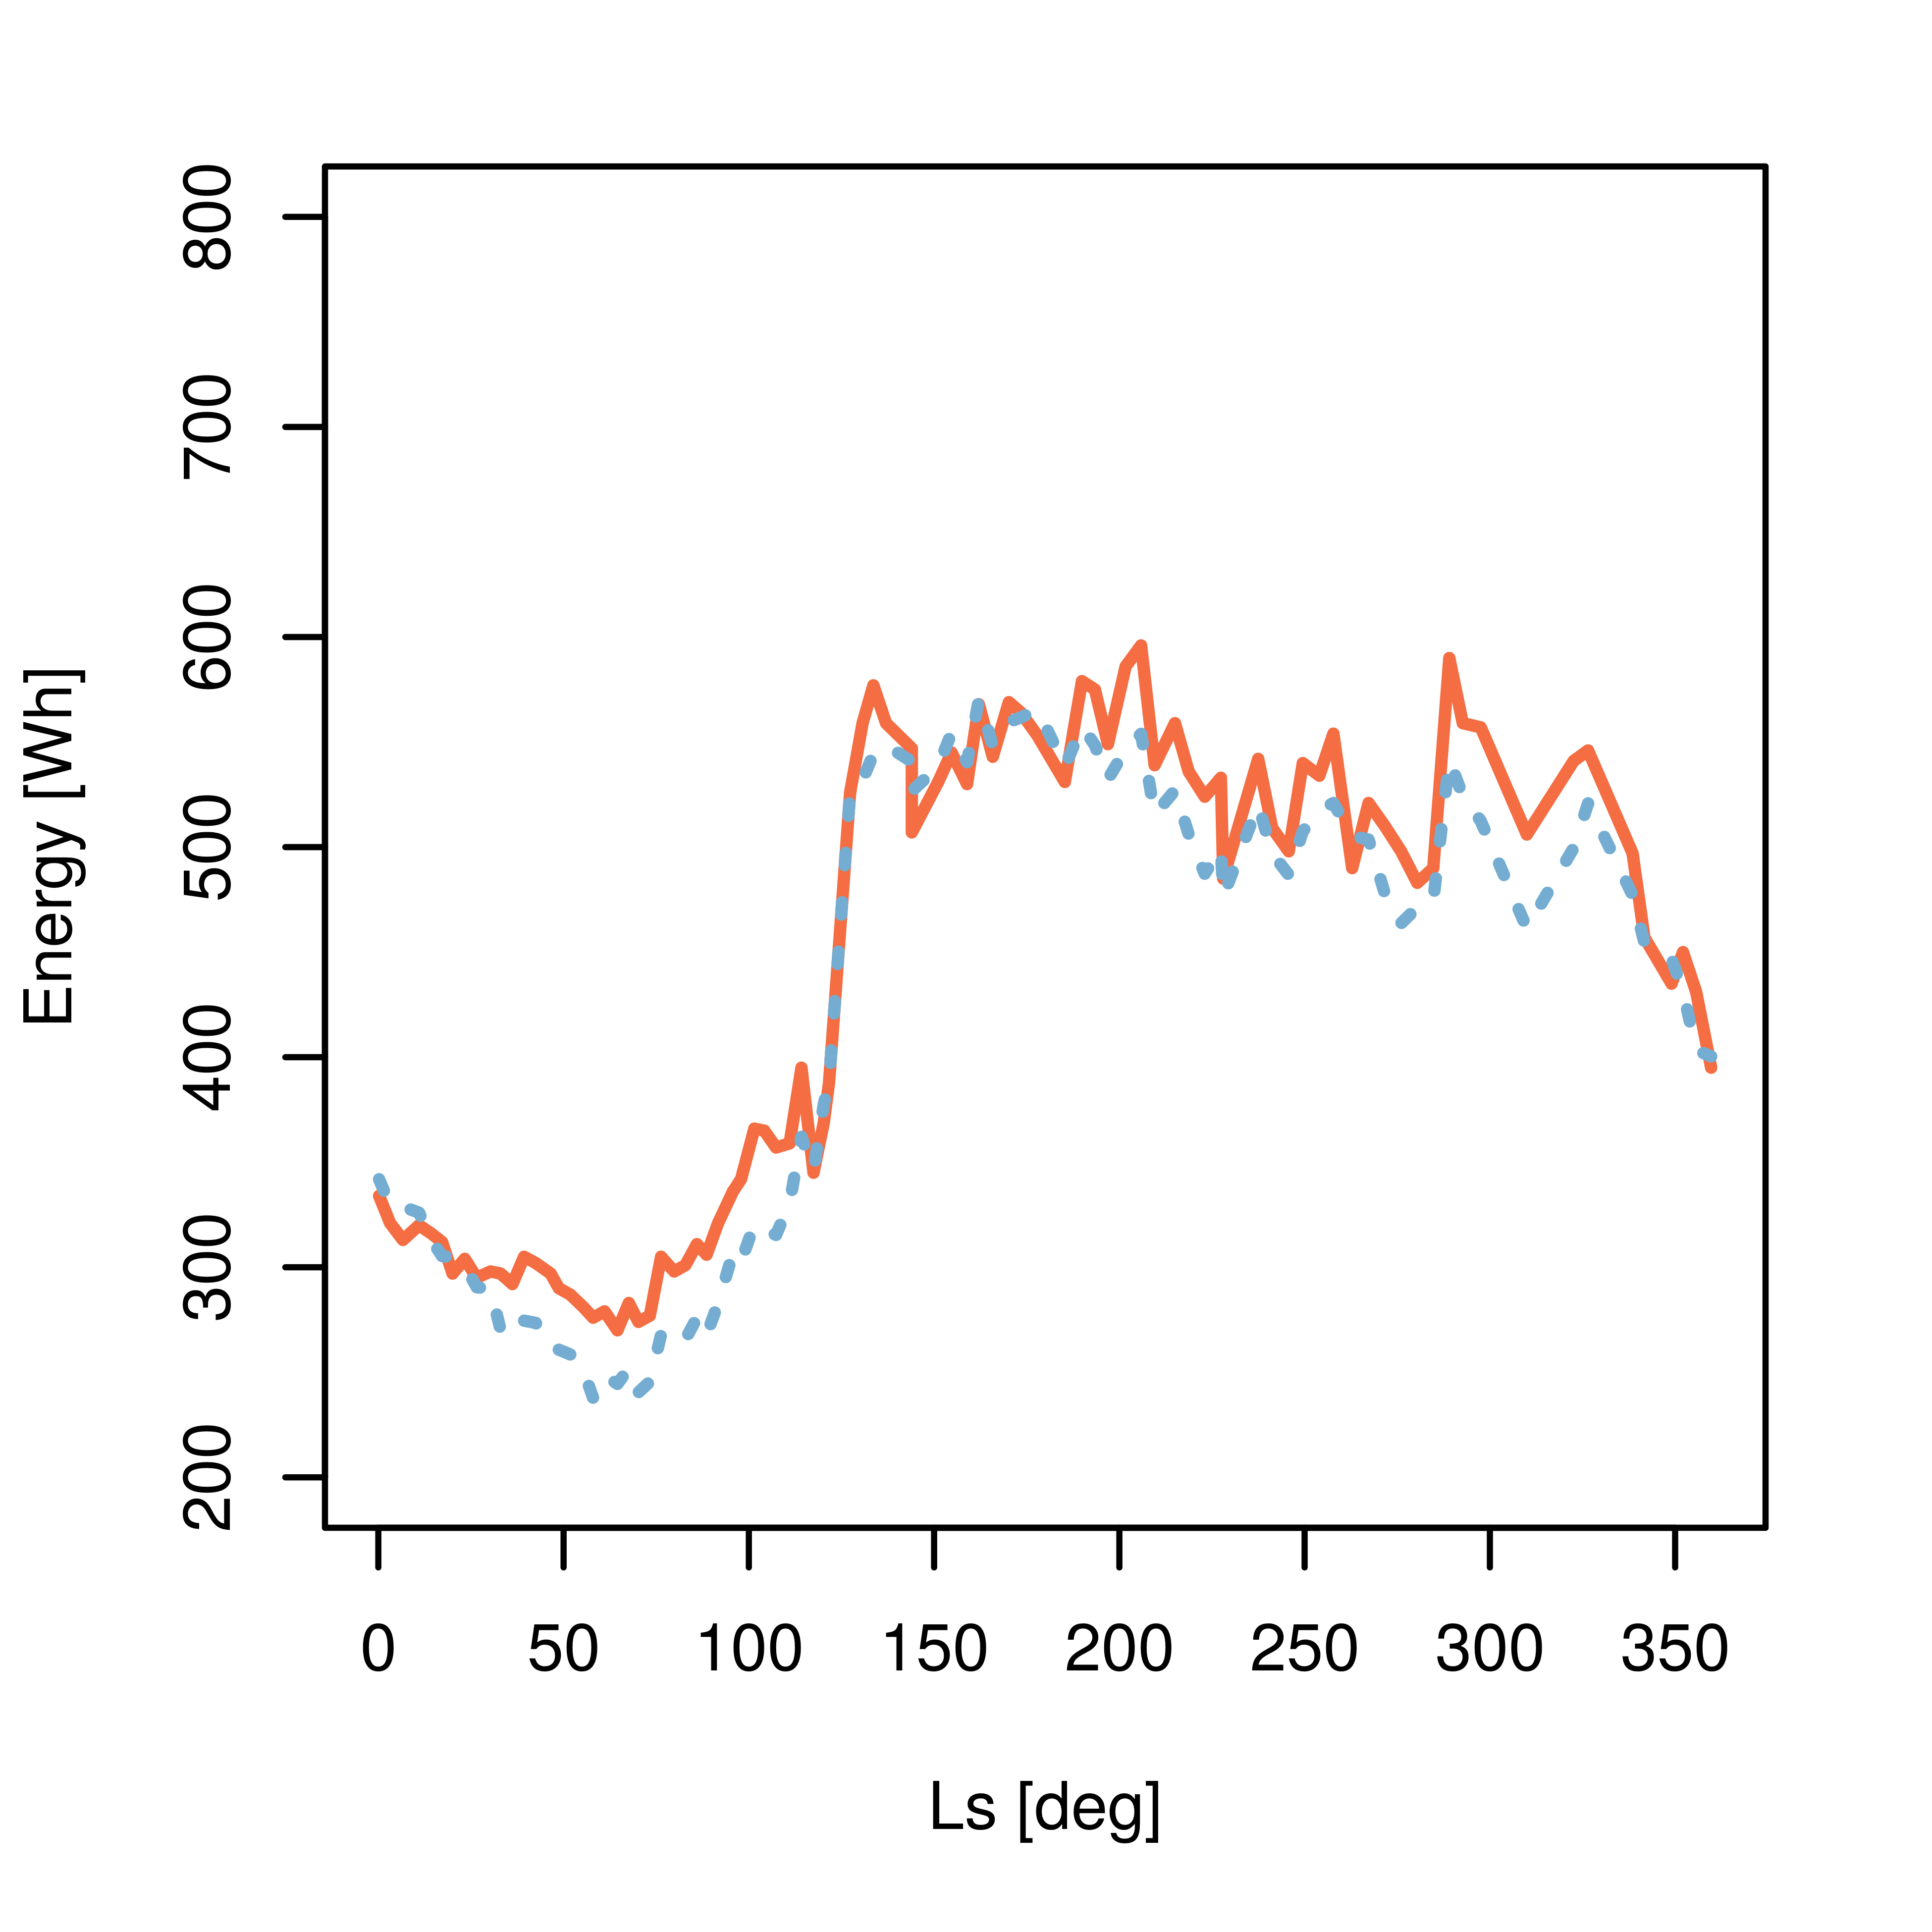
\includegraphics[height=\graphicsHeight]{sections/appendix/energy-error-margin/plots/predicted-vs-measured-energy-my30-adjusted-without-outliers.png}
		\subcaption{MY30}
		\label{fig:plot:sub:mer-energy-production-predicted-vs-reported-my30-adjusted-without-outliers}
	\end{subfigure}\hfill
    \begin{subfigure}[t]{\subfigureWidth}
        \centering
		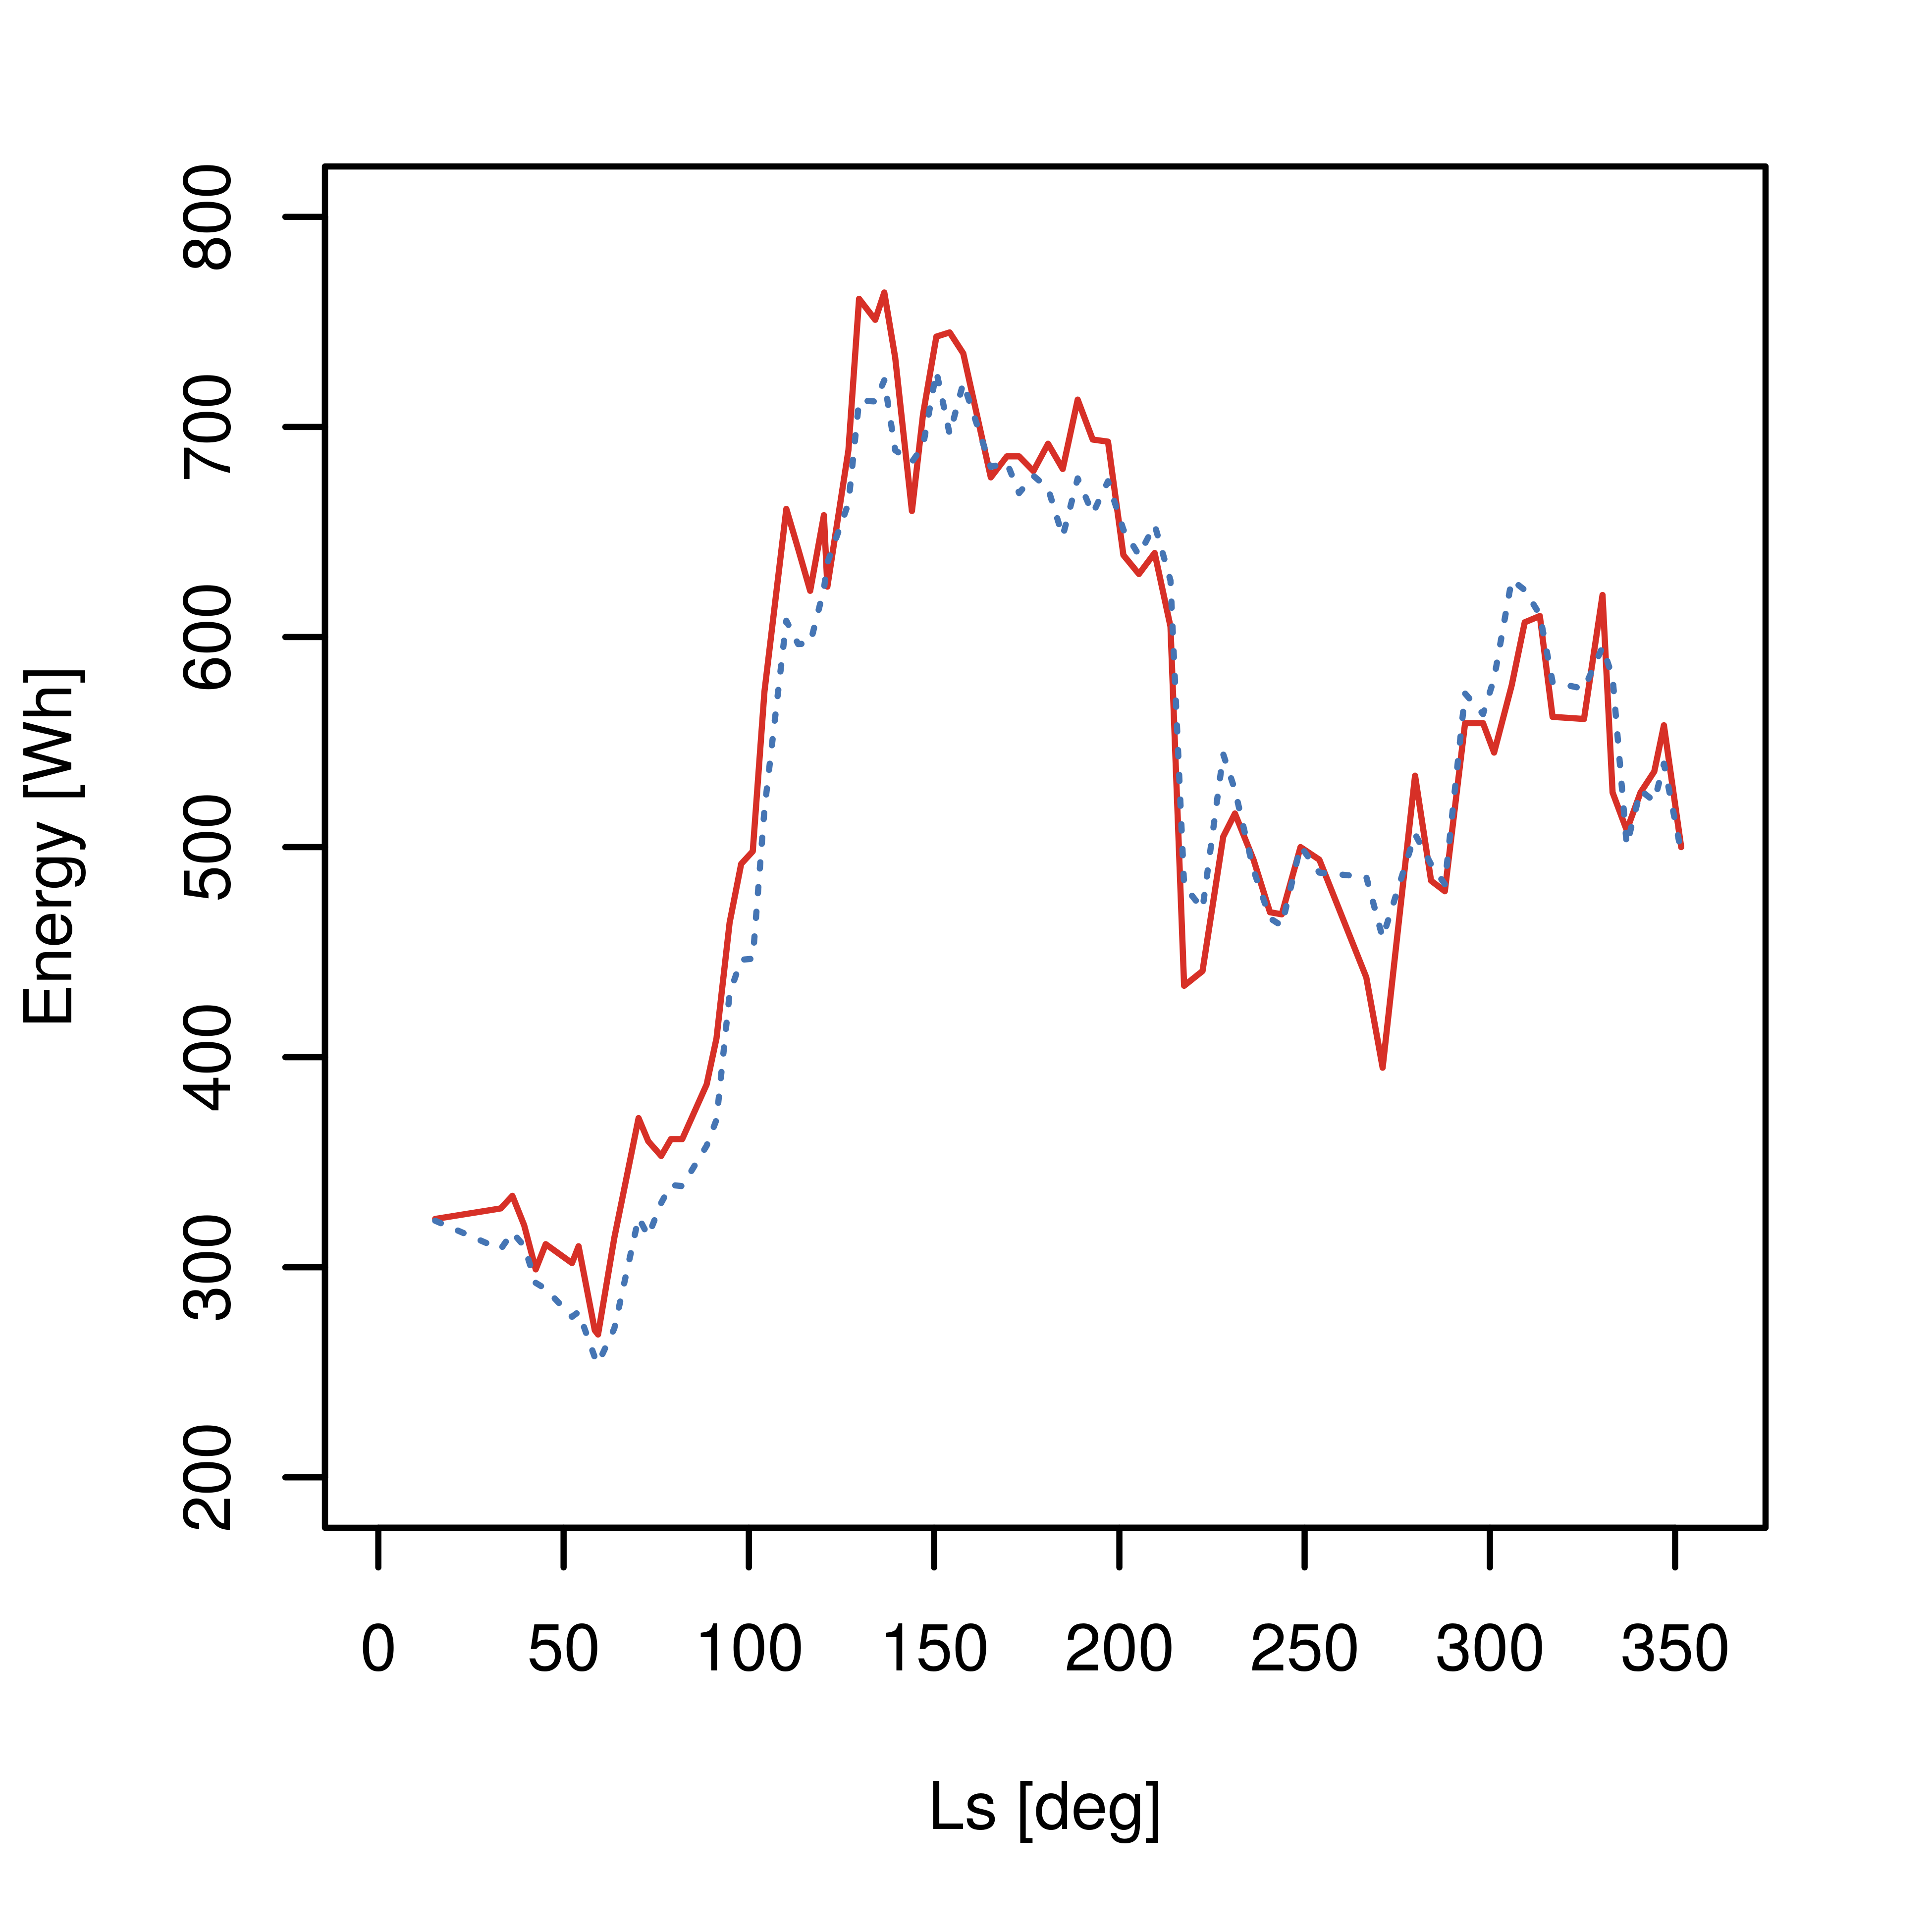
\includegraphics[height=\graphicsHeight]{sections/appendix/energy-error-margin/plots/predicted-vs-measured-energy-my32-adjusted-without-outliers.png}
		\subcaption{MY32}
		\label{fig:plot:sub:mer-energy-production-predicted-vs-reported-my32-adjusted-without-outliers}
	\end{subfigure}
    \caption[\ac{MER} Opportunity \ac{PV} energy production: adjusted prediction vs reported]
            {\ac{MER} Opportunity \ac{PV} energy production: adjusted prediction vs reported. The predicted lines across the first row were obtained with iteratively determined calculation adjustments that narrowed the calculated predicted values' error margin range from -33\%/+7\% to -10\%/+25\%. The second row was obtain in a similar fashion but with outlier divergences ignored which further narrowed the error margin range to -11\%/+5\%.}
    \label{fig:plot:mer-energy-production-predicted-vs-reported-adjusted-with-and-without-outliers}
\vspace{-2ex}
\end{figure}

\clearpage
